\documentclass{beamer}

%%% -------------- CREATE HANDOUTS -----------------------------------
%\documentclass[12pt, handout]{beamer}
%\usepackage{pgfpages}
%\pgfpagesuselayout{4 on 1}[letterpaper, landscape, border shrink=5mm]
%%% ------------------------------------------------------------------


\mode<presentation>
  \usepackage{ru}
  %\usetheme{Warsaw}
  %\usecolortheme{seahorse}
  %\usefonttheme{default}
  \setbeamertemplate{caption}[numbered]
  %\setbeamertemplate{navigation symbols}{}
  \setbeamertemplate{bibliography item}[text]
\setbeamertemplate{headline}{}
\newcommand*\oldmacro{}%
	\let\oldmacro\insertshorttitle%
%\renewcommand*\insertshorttitle{%
%   \oldmacro\hfill%
%   \insertframenumber\,/\,\inserttotalframenumber}
\setbeamertemplate{section page}{
    \begin{centering}
    \vspace{1cm}
    \begin{beamercolorbox}[rounded=true,shadow=false,sep=4pt,center]{part title}
    \usebeamerfont{section title}\LARGE{\insertsection}\par
    \end{beamercolorbox}
    \end{centering}}
\usepackage{ragged2e}
\usepackage[english]{babel}
\usepackage[utf8]{inputenc}
\usepackage{appendixnumberbeamer}
\usepackage{natbib}
\usepackage{textpos}
\usepackage{lipsum}
\usepackage{tikz}
\usepackage[percent]{overpic}
\usepackage{textcomp}
\usepackage{booktabs}
\usepackage{mathabx}
\usepackage{pifont}
\usepackage{bbding}
\usepackage{fontenc}
%\let\Sun\undefined   %to undefine something
%\usepackage{marvosym}
%\usepackage{scalerel}
%% \usepackage[
%%   style=numeric,
%%   citestyle=authoryeartitle
%% ]{biblatex}
\setbeamerfont{caption}{size=\tiny}


% define ``struts'', as suggested by Claudio Beccari in
%    a piece in TeX and TUG News, Vol. 2, 1993.
\newcommand\Tstrut{\rule{0pt}{2.6ex}}         % = `top' strut
\newcommand\Bstrut{\rule[-0.9ex]{0pt}{0pt}}   % = `bottom' strut



%\setbeameroption{show notes}
%\setbeamertemplate{note page}[plain]
\newcommand{\tss}{\textsuperscript}
\newcommand{\tsbs}{\textsubscript}
%Change Bullets in latex list
\setbeamertemplate{itemize item}{\scriptsize\raise1.25pt\hbox{\donotcoloroutermaths\ding{118}}}
\setbeamertemplate{itemize subitem}{\scriptsize\raise1.25pt\hbox{\ding{226}}}
\setbeamertemplate{itemize subsubitem}{\tiny\raise1.25pt\hbox{\ding{169}}}
\setbeamertemplate{enumerate item}{\insertenumlabel.}


%%To select specific font
%{\fontsize{2.5}{4}\selectfont tobesize}

%\setbeamertemplate{background}{\tikz[overlay, remember picture]\node[xshift=-2.3cm, yshift=1.50cm, opacity=0.4]at (current page.south east){
\includegraphics[width=4cm]{images}};}

\title[Program Progress]{Program Progress}
\author{Paul Mendoza}
\date{March 8, 2016}

\begin{document}
\setbeamertemplate{caption}{\raggedright\insertcaption\par}
\begin{frame}
	%% background
  %% \tikz[overlay, remember picture]\node[xshift=-3.5cm, yshift=3cm, opacity=0.1]at (current page.south east){
\includegraphics[width=8cm]{tamu_system_proposed_seal_042915}};
	%% Left-hand logo
  %% \begin{tikzpicture}[remember picture, overlay]
  %% \node [xshift = 3 cm, yshift=1.2cm] at (current page.south west){
\includegraphics[width=5cm]{tees_logo_primary_maroon}};
  %% \end{tikzpicture}
    %% Right-hand logo
  %% \begin{tikzpicture}[remember picture, overlay]
  %% \node [xshift = -3cm, yshift=1.2cm] at (current page.south east){
\includegraphics[width=5cm]{TEES_NSSPI_logo_HMaroon}};
  %% \end{tikzpicture}
  %% Upper logo right
    %% \begin{tikzpicture}[remember picture,overlay]
    %% \node[anchor=north east,yshift=2pt] at (current page.north east) {
\includegraphics[height=0.8cm]{NUENlogo}};
    %% \end{tikzpicture}
  %% Upper logo left
    %% \begin{tikzpicture}[remember picture,overlay]
    %% \node[anchor=north west,yshift=2pt] at (current page.north west) {
\includegraphics[height=0.8cm]{NUENlogo}};
    %% \end{tikzpicture}
    \titlepage
    \vspace{-1.8cm}
    \begin{center}
      Presented at Research Meeting
    \end{center}
\end{frame}

%Add Biola Seal
%% \setbeamertemplate{background}{\tikz[overlay, remember picture]\node[xshift=-2.5cm, yshift=2.5cm, opacity=0.05]at (current page.south east){
\includegraphics[width=6cm]{imageedit_2_7317234434}};}

%Add NSSPI to upper right
%% \addtobeamertemplate{frametitle}{}{%
%%   \begin{tikzpicture}[remember picture,overlay]
%%     \node[anchor=north east,yshift=2pt] at (current page.north east) {
\includegraphics[height=0.8cm]{TEES_NSSPI_Acronym_logo_WHT}};
%%     \end{tikzpicture}}



%% \begin{frame}{Outline}
%% \tableofcontents
%% \end{frame}

\begin{frame}%{Analytical Procedure}
  \begin{figure}[H]
    %\vspace{-3mm}
    \begin{center}
      \hbox{\hspace{2.5cm}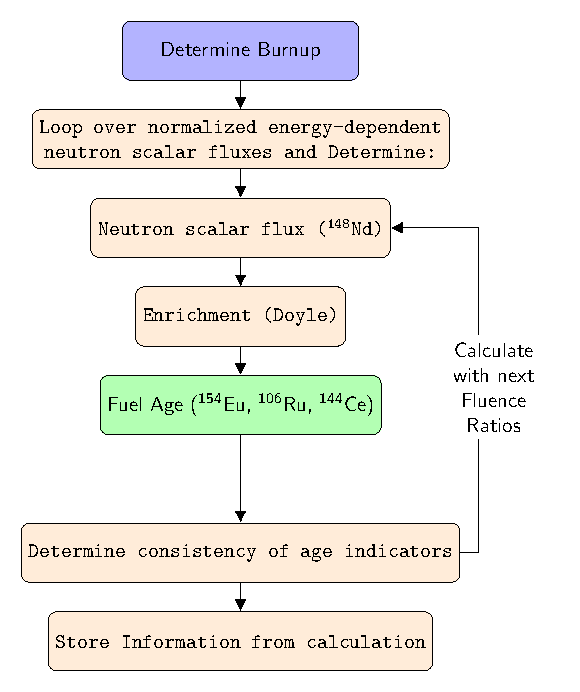
\includegraphics[scale = 0.7]{figures/android.pdf}}
    \end{center}
  \end{figure}  
\end{frame}      


%% \begin{frame}{Analytical Procedure}
%%   \begin{equation*}
%%     \frac{dn_i}{dt}=-\lambda_i^{eff}n_i+
%%     \sum_{j=1}^{N}b_{j\rightarrow i}^{eff}n_j
%%   \end{equation*}
%%   \begin{equation*}
%%     \lambda_i^{eff}=\lambda_i+\phi\sum_{j=1}^N\sigma_{i\rightarrow j}
%%   \end{equation*}
%%   \begin{equation*}
%%     b_{j\rightarrow i}^{eff}=b_{j\rightarrow i}\lambda_j+
%%       \sigma_{j\rightarrow i}\phi+\gamma_{j\rightarrow i}\sigma_{j,f}\phi
%%   \end{equation*}
%%   \begin{equation*}
%%     \frac{d\vec{n}}{dt}=\bm{A}\vec{n}(t)\rightarrow\vec{n}=e^{\bm{A}t}\vec{n}_0
%%   \end{equation*}
%%   %% %The solution to this system is so obvious, I won't even write it down.
%%   %% \begin{equation*}
%%   %%   \vec{n}=e^{\bm{A}t}\vec{n}_0
%%   %% \end{equation*}
%% \end{frame}



\section{Flux Spectrum}
%% \begin{frame}{Flux Spectrum}
%%   \begin{itemize}
%%   \item{Example flux spectra}
%%   \item{Equations for flux spectra, Ratios, etc}
%%   \end{itemize}
%% \end{frame}

\begin{frame}{Cross-section calculations}

  \begin{equation*}
    \sigma=\frac{\int\sigma(E)\phi(E)dE}{\int\phi(E)dE}
  \end{equation*}

  \begin{align*}
    \phi(E) =& C_1\cdot \frac{E}{E_0^2} \cdot
    exp\left(-\frac{E}{E_0}\right) &&E<E_{max,th}\\
    =& \frac{C_2}{E}  &&E_{max,th}<E<E_{max,epi}\\
    =& C_3 \cdot \frac{\sqrt{\frac{E}{E_f}}}{E_f}
    \cdot exp\left(-\frac{E}{E_{f}}
    \right) &&E>E_{max,epi}
  \end{align*}


  {\tiny
    \setlength{\abovedisplayskip}{6pt}
    \setlength{\belowdisplayskip}{\abovedisplayskip}
    \setlength{\abovedisplayshortskip}{0pt}
    \setlength{\belowdisplayshortskip}{3pt}
    \begin{align*}
      C_1=&\frac{E_0^2}{E^2_{max,th}}e^{E_{max,th}/E_0}
      \\
      C_2=&1\\
      C_3=&\frac{E_f}{E_{max,epi}}
      \cdot
      e^{\frac{E_{max,epi}}{E_f}}\frac{1}
      {\sqrt{\frac{E_{max,epi}}{E_f}}}
    \end{align*}
    }%
  {\tiny
  $E_{max,th}=0.50\ \text{eV}$,
  $E_{max,epi}=1E5\ \text{eV}$,
  $\theta_{th}=0.09\ \text{eV}$ (764 K),
  $\theta_{fis}=1.35E6\ \text{eV}$}%
\end{frame}

\begin{frame}
      \begin{figure}[H]
        \vspace*{-1cm}
        \begin{center}
          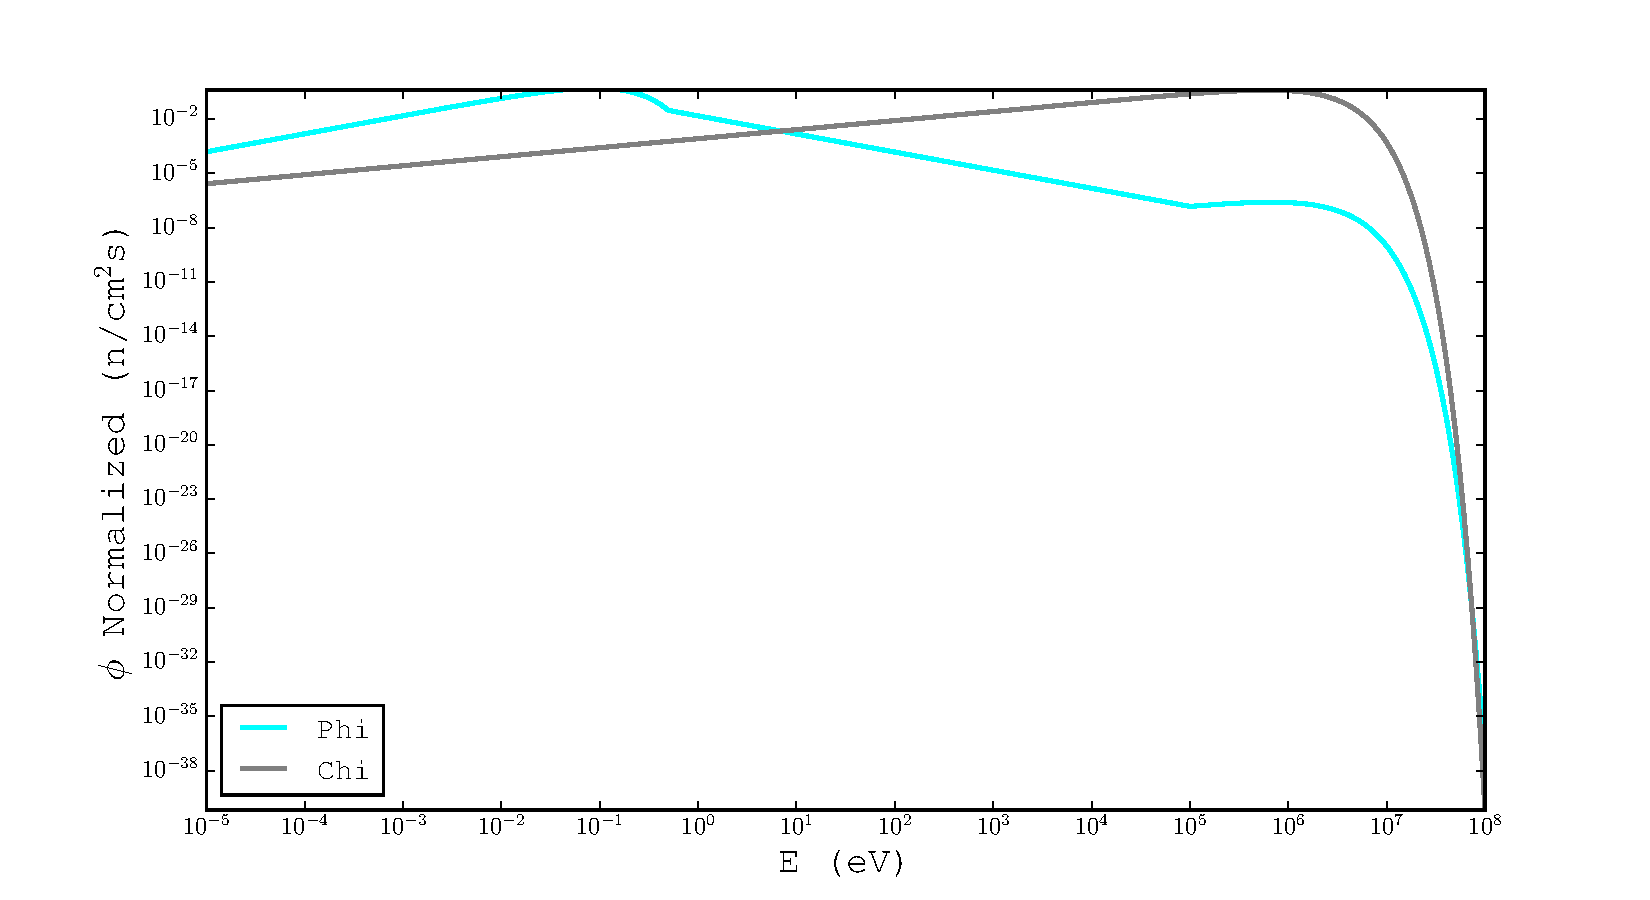
\includegraphics[scale = 0.4]{../../Calculations/Project/Weighting/Figures/Phi_N_Chi.pdf}
          \vspace{-0.5cm}
        \end{center}
      \end{figure}
      \vspace{2cm}
      \begin{equation*}
        \chi=C_4e^{-\frac{E}{a}}sinh\left(\sqrt{bE}\right)
      \end{equation*}
\end{frame}


\begin{frame}{Bateman Results}
  \begin{columns}
    \begin{column}{0.5\textwidth}
      \begin{figure}[H]
        \vspace*{-1cm}
        \begin{center}
          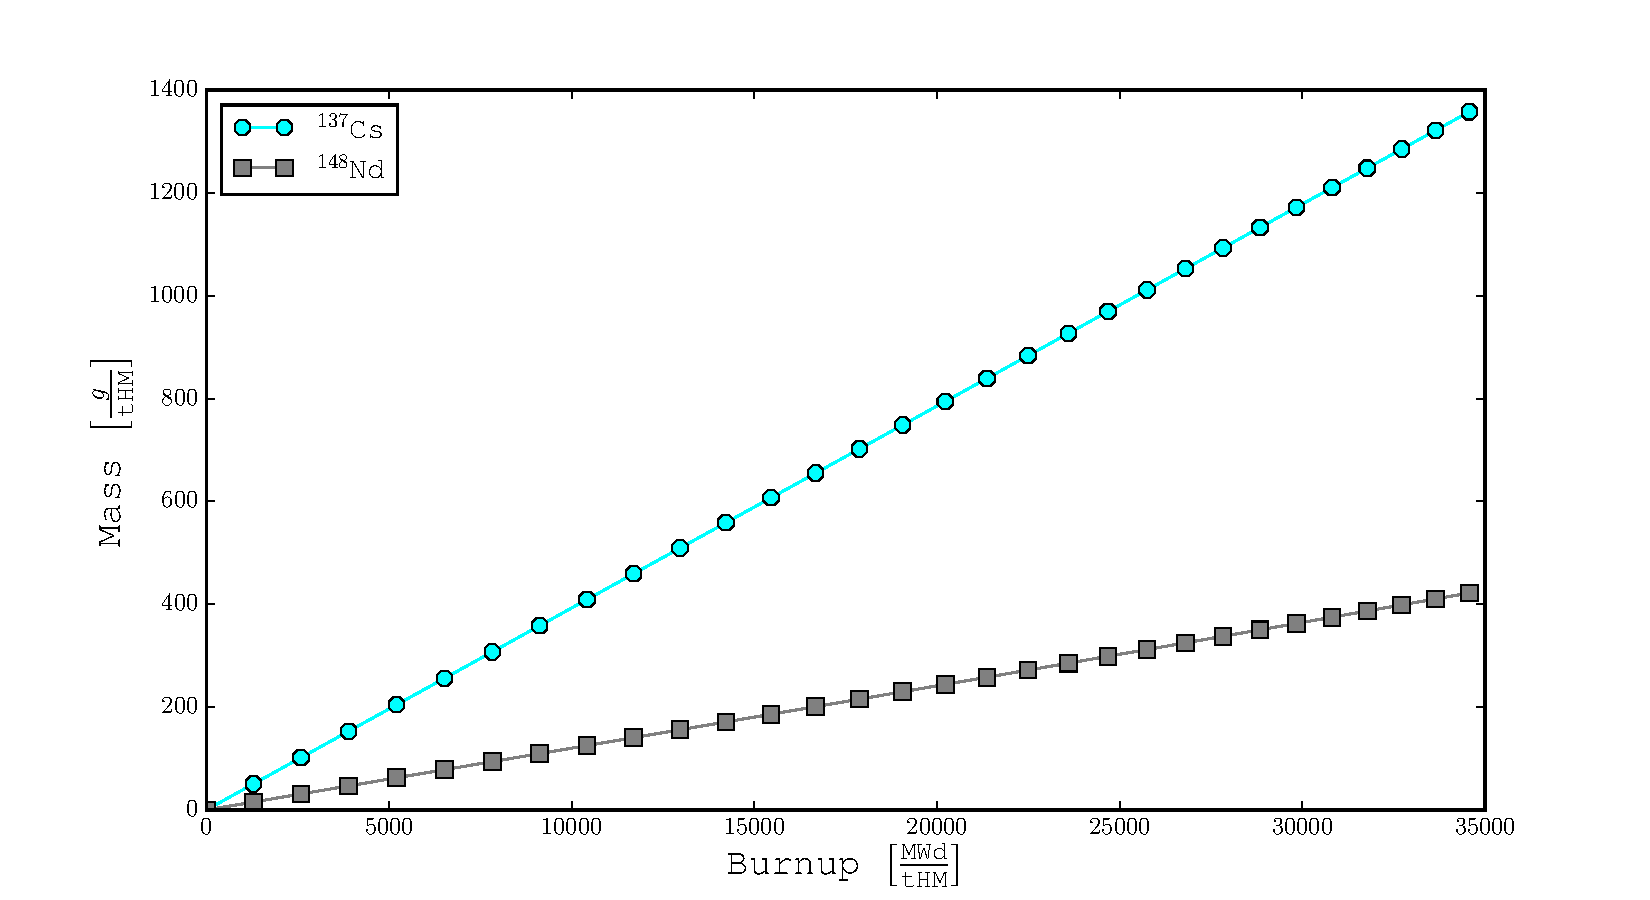
\includegraphics[scale = 0.4]{../../Calculations/Bateman/PlotBU/Plots/BurnCsComp_grams.pdf}
          \vspace{-0.5cm}
        \end{center}
      \end{figure}
    \end{column}
    \begin{column}{0.5\textwidth}
    \end{column}
  \end{columns}  
\end{frame}


\section{Cross Sections}

\begin{frame}{One Group Cross Section Comparison}
  \vspace{-4mm}
  \begin{table}[H]
  \begin{center}
    \resizebox{\textwidth}{!}{%
    \begin{tabular}{l l l l}
      \toprule
      Isotope\tss{Rxn} & ENDF VII & ORIGEN2 & Ratio\Tstrut\Bstrut\\
      \hline
      \tss{239}Pu\tss{$\gamma$} & 6.544e+01 & 6.909E+01 & 1.06\Tstrut\\
      \tss{240}Pu\tss{$\gamma$} & 1.521e+02 & 2.228E+02 & 1.46\\
      \tss{241}Pu\tss{$\gamma$} & 4.518e+01 & 4.202E+01 & 0.93\\
      \tss{235}U\tss{$\gamma$}  & 9.387e+00 & 1.068E+01 & 1.14\\
      \tss{238}U\tss{$\gamma$}  & 4.098e+00 & 8.872E-01 & 0.22\\
      \tss{239}Pu\tss{f} & 1.179e+02 & 1.211E+02 & 1.03\\
      \tss{240}Pu\tss{f} & 9.609e-01 & 5.787E-01 & 0.60\\
      \tss{241}Pu\tss{f} & 1.253e+02 & 1.259E+02 & 1.01\\
      \tss{235}U\tss{f}  & 4.621e+01 & 4.752E+01 & 1.03\\
      \tss{238}U\tss{f}  & 2.091e-01 & 9.281E-02 & 0.44\\
      \bottomrule
    \end{tabular}}
  \end{center}
  \end{table}
\end{frame}

\begin{frame}{ORIGEN2 Model}
  \begin{center}
    $
    \frac{552.8\ \text{g \tss{137}Cs}}{Mt}\cdot
    \frac{6.022E23\ \text{atoms}}{137\ \text{g \tss{137}Cs}}\cdot
    \frac{\text{Fission}}{0.06\ \text{atoms}}\cdot
    \frac{200\ \text{MeV}}{\text{Fission}}\cdot
    \frac{1.602E-19\ \text{MJ}}{1\ \text{MeV}}\cdot
    \frac{1\ \text{day}}{86400\ \text{s}}=15,018\ \frac{\text{MWd}}{Mt}$
  \end{center}
\end{frame}



\section{Bateman Results}
\begin{frame}{Constant Power}
  From ORIGEN 2.2 calculation
  \begin{equation*}
    \phi=\frac{6.242\cdot10^{18}\cdot P}{\sum_i \chi_i^f\sigma_i^fR_i}
  \end{equation*}
  $\phi$=instantaneous neutron flux\\
  $P$=power (MW)\\
  $\chi_i^f$=amount\\
  $\sigma_i^f$=microscopic fission cross section for nuclide $i$\\
  $R_i$=recoverable energy per fission for nuclide $i$ (MeV/fission)
  \begin{equation*}
    R_i\text{MeV/Fission}=1.29927x10^{-3}(Z^2A^{0.5})+33.12
  \end{equation*}
\end{frame}

\begin{frame}{Bateman Results}
  \begin{columns}
    \begin{column}{0.5\textwidth}
      \begin{figure}[H]
        \vspace*{-1cm}
        \begin{center}
          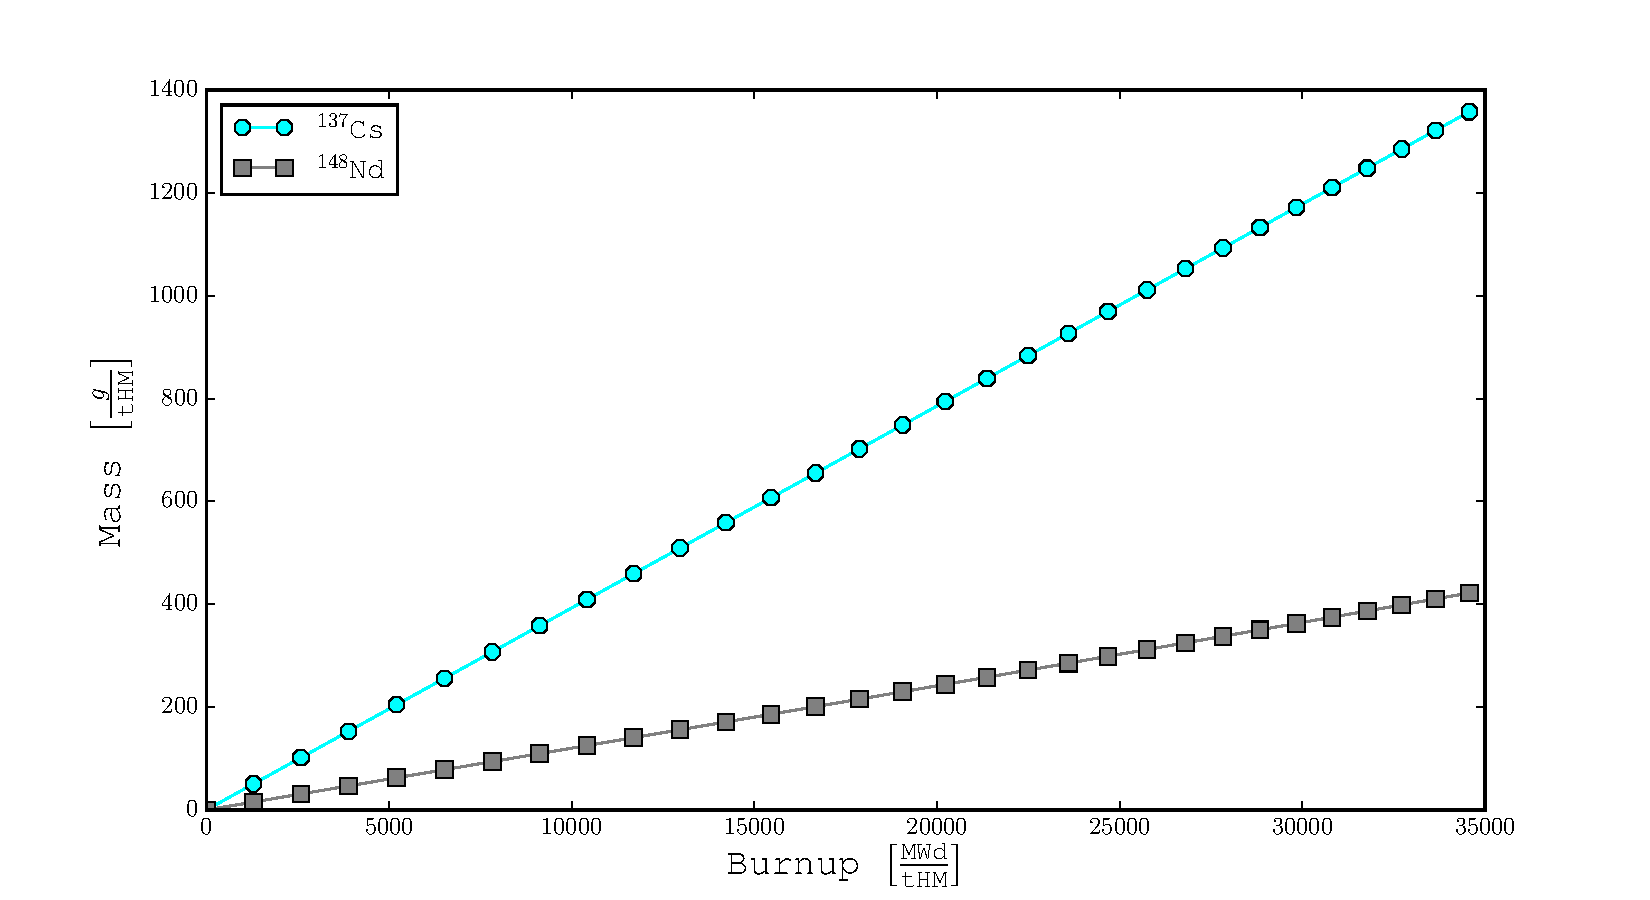
\includegraphics[scale = 0.4]{../../Calculations/Bateman/PlotBU/Plots/BurnCsComp_grams.pdf}
          \vspace{-0.5cm}
        \end{center}
      \end{figure}
    \end{column}
    \begin{column}{0.5\textwidth}
    \end{column}
  \end{columns}  
\end{frame}





\section{Next Week}
\begin{frame}{Next Week}
  \begin{itemize}
  \item{All the x-sections}
  \end{itemize}
\end{frame}

\end{document}
